\documentclass[12pt, letterpaper]{article}
\usepackage[margin=0.8in]{geometry}
\usepackage[utf8]{inputenc}
\usepackage[numbers]{natbib}
\usepackage{graphicx}
\usepackage{xcolor}
\usepackage{wrapfig}

\usepackage{hyperref}

\title{CMSC499A: Interactive Mutation Signature Explorer}
\author{Mark Keller \thanks{advised by Professor Max Leiserson}}
\date{Spring 2018}

\begin{document}
\maketitle

\begin{abstract}
Identification and analysis of patterns in data can be difficult without visualization tools. 
Datasets of somatic mutations in cancer are no exception.
Recent whole-genome sequencing projects have produced large amounts of mutation data to be explored.
Of great importance is the classification of different mutational processes and the mutational signatures \citep{alexandrov2013signatures} they leave behind.
As new mutational signatures continue to be discovered, observation of the levels of signature activity, called signature exposure, helps show how the underlying mutational processes differ across cancer types, time, and environmental variables.
Visualizations of mutational signatures and mutation datasets in the context of these variables can help researchers to quickly observe trends and relationships in this data, verifying current knowledge or prompting further analysis.
This paper describes a mutation visualization tool developed this semester that allows simple somatic mutation datasets and mutation signatures to be explored interactively and provides users with publication-ready graphics.
\end{abstract}

\section{Introduction}
% Background about mutational signatures
Mutation signatures are distinctive patterns of somatic mutations generated by different mutational processes over the course of a lifetime \citep{alexandrov2013signatures}.
Deamination, a biochemical reaction that removes an amine group from a molecule, is one process that has been linked to several mutational signatures \citep{helleday2014mechanisms}.
These patterns have been extracted from mutation datasets using computational and mathematical techniques \citep{alexandrov2013deciphering}.
The concept of mutational signatures has been validated by in vitro experiments that perform knockouts of DNA repair genes and then observe that mutational signatures result \citep{zou2018validating,nik2015genome}.

% Importance of mutational signatures
Observation of mutational signatures and knowledge of the mutational processes that cause them can improve cancer diagnosis and treatment. 
Mutational signatures have been used to predict deficiency of BRCA1 and BRCA2, genes that produce tumor suppressor proteins \citep{domchek2010association}.
Knowledge of such deficiencies in breast cancers can allow therapeutic response to be predicted as early as the first biopsy \citep{davies2017hrdetect}.
In colorectal cancers, mutational signatures have enabled identification of base excision repair (BER) defects \citep{pilati2017mutational}. 
BER is a repair process that enables altered DNA bases to be recognized and removed, with defects in this process causing multiple mutation patterns to arise \citep{helleday2014mechanisms}.
Being able to attribute genomic instability to BER can prompt genetic counselling and immunotherapy measures that take into consideration a particular mutation load \citep{pilati2017mutational}.

% Current questions
There are many open questions about mutational signatures. 
Currently, mutational signatures are represented as probability distributions over 96 categories of single-nucleotide variant (SNV) mutations.
These 96 categories include the reference base, the variant base, and one flanking base pair in each direction. 
It is not known how significant these flanking base pairs are, how many to consider, or to what extent these depend on one another \citep{shiraishi2015simple}.
The mutational processes that cause some of the currently published mutational signatures remain unknown \citep{alexandrov2013signatures}.
Methods to consider other types of mutations (indels and rearrangements) are only being formulated now \citep{zou2018validating}.

% Existing visualizations/browsers
Many interactive cancer visualization tools and browsers exist, but few consider or provide support for mutational signatures. 
For example, the cBio Cancer Genomics Portal provides interactive visualizations of mutation data with a focus on copy number alterations, mRNA expression changes, DNA methylation values, and protein and phosphoprotein levels \citep{cerami2012cbio,gao2013integrative}.
The cBio Portal also contains features for computing mutual exclusivity and co-occurrence between pairs of genes \citep{cerami2012cbio,gao2013integrative}.
The UCSC Xena Browser supports gene, exon, miRNA and protein expression, copy number, DNA methylation and somatic mutation data along with phenotypes, subtype classifications and genomic biomarkers \citep{goldman2014ucsc,goldman2016ucsc}.
FireBrowse is a cancer data browser that does include plots of mutation signature exposure that can be compared to clinical data, but only includes 5 signatures for analysis.
It is unclear what these 5 signatures represent or if any of these are related to any of the widely-used signatures published by Catalogue Of Somatic Mutations In Cancer (COSMIC).
\subsection{Contributions}
A browser that can easily visualize mutation datasets and contributions of the over thirty currently known mutational signatures is needed, as it could allow trends and relationships with clinical data to be spotted easily.
This could further understanding of the underlying mutational processes that cause certain signatures to be expressed.

% Introduction to iMuSE
Interactive Mutation Signature Explorer (iMuSE) is a web-based (\url{https://imuse.lrgr.io}) mutation data browser that enables exploration of mutational signatures, SNV mutations, and mutation density.
This tool allows users to choose sequencing project datasets by cancer type, as well as mutational signature combinations (of which can be selected based on cancer-type-specific presets) before plotting this data. 
Web-based interactive visualizations allow for exploration across datasets and features in a way that is accessible and fast.
Data exploration through these visualizations can be used to make initial inferences that lead to further statistical analysis, or, alternatively, can be used to verify and communicate relationships found through prior analysis.

% Types of visualizations
Each type of visualization produced by iMuSE aims to enable further examination of a trend or relationship which has been hypothesized or presented in existing literature.
The following are types of visualizations that can be generated and their motivations:
\begin{enumerate}
\item It is well known that tobacco and alcohol usage increases risk of many types of cancers \citep{doll1956lung,collaborative2002alcohol}. A question of interest is how mutational signatures relate to smoking status and other clinical variables. \citet{alexandrov2016mutational} finds that smokers exhibit increases in mutations attributed to COSMIC signatures 2, 4, 5, 13, and 16. \citet{kim2016somatic} also notes an association between signature 5 and smoking.

To illustrate estimated contributions of a selected combination of mutational signatures, a stacked bar plot can be generated, showing estimated signature exposures for a sample, along with tobacco and alcohol usage indicators.
Exposure values can be normalized to sum to one for each sample, or kept relative to the total number of mutations in each sample.
This plot type was inspired by Figure 4 in \citet{kim2016somatic} that displays estimated contributions of 4 different signatures and tobacco usage over cohorts of urothelial cancer tumor samples.
    
\item Localized hypermutation, known as kataegis, was first discussed by \citet{taylor2013dna}, in which whole-genome sequencing of breast cancers showed regions with mutation ``rainfalls" - greater than 5 mutations with significantly short intermutational distances. Mutations in regions of kataegis have been shown to occur frequently at C base pairs preceded by a 5-prime T base pair, due to APOBEC activity during double-strand break repair \citep{taylor2013dna,alexandrov2013signatures}. Since this introduction in 2013, kataegis has been shown to occur in additional tumor types \citep{alexandrov2013signatures}. COSMIC signatures 2 and 13 have been associated with APOBEC activity, and by extension, kataegis \citep{alexandrov2013signatures}. There is recent interest in rigorous statistical identification and verification of kataegis \citep{yousif2018origins}.

To examine mutation clusters, specifically those occurring in regions of kataegis, a rainfall plot can be generated for each sample.
Mutations are plotted horizontally based on their genome location, and vertically by the distance (in bp) to the previous mutation.
Mutations are colored according to one of 96 mutation categories (5' flanking base pair, single-nucleotide variant, 3' flanking base pair).
Rainfall plots are commonly used to examine regions of hypermutation, as they allow these regions to be easily identified by tight vertical clusters of mutations. 
Similar rainfall plots can be seen in Figure 4 of \citet{nik2012mutational} and in Figure 6 of \citet{alexandrov2013signatures}.

To identify samples containing instances of localized hypermutation, kataegic events can be highlighted along the genome in a second type of plot.
Along the vertical axis are samples, and along the horizontal axis is the genome.
Users can zoom and pan along each chromosome, and easily pinpoint kataegis events by the dark bars located on mutations in kataegis regions.
Samples are grouped by sequencing project and cancer type.
This plot acts as a rainfall plot selector, as each sample bar can be clicked to generate a corresponding rainfall plot.
To our knowledge, this style of plot has not been used before to visualize kataegis .
    
\item A question that prompted the development of this visualization tool is whether certain mutational signatures are associated with mutations in specific genomic locations or regions.
One way to examine this is to look at mutation signature activity across the genome with a ``Manhattan plot".
The Manhattan plot gets its name from the resemblance of a skyline along the genome, and is typically used to visualize the output of statistical significance tests used in genome-wide association studies \citep{gibson2010hints}.
To generate this plot, signatures are assigned to individual mutations (see Methods section for details) and then grouped into bins by chromosome location and signature.
The horizontal axis represents the genome location, and the vertical axis represents the number of mutations within a bin.
To our knowledge, this is a new method for exploring mutational signatures along the genome.

\end{enumerate}

The rest of this paper is organized into the following sections: Methods, Case Studies, and Conclusions. Included in the Methods section are discussions of open-source libraries and frameworks used to create the browser application, the steps taken to process raw mutation and clinical datasets and the sources of these datasets, and the algorithms used to compute signature exposures. The Case Studies section presents two use cases for this tool: exploration of the relationship between alcohol usage and mutational signatures, and verification of the mutation categories typically present in regions of hypermutation. Future directions for development of iMuSE are outlined in the Conclusions section.


\section{Methods}
\subsection{Data}
Data processing for plots occurs in two stages. 
Simple somatic mutation datasets and donor clinical datasets from sequencing projects are downloaded and processed into a uniform format. 
This conversion must be specified for each sequencing project, as each provides datasets in a different format.
Currently, processing has been completed for simple somatic mutation and clinical datasets from the Pan-Cancer Analysis of Whole Genomes (PCAWG) study.
Once into a uniform format, these datasets are stored in a bucket in the UMIACS object store, and can be processed dynamically by a web server as specific requests are made for visualizations.
Usage of the object store allows future developers to quickly get the application up and running without needing to perform this initial time-consuming data processing step.
Dynamic processing is performed by a web application written in Python with the Flask framework. 
The Pandas and NumPy packages are used for data manipulation in both of these processing stages.

\subsection{Exposures}
Signature exposures are estimated using a quadratic programming approach detailed by \citet{huang2017detecting}.
To generate the aforementioned Manhattan Plot showing signatures across the genome, signatures are assigned to mutation categories for each sample by first computing estimated signature exposures, then taking the maximum of the product of each signature's probability for the mutation category and the sample's exposure to the same signature.
Signatures present in each cancer type, or signature combination ``presets", are based on those specified in publications of mutational signatures.
For example, the presences of COSMIC signatures can be found in Figure 3 of \citet{alexandrov2013signatures}.

\subsection{Implementation and Availability}
% Frameworks and libraries used
Using the Vue JavaScript framework, the application is made up of reusable components that encapsulate templates, functions, and variables.
This encapsulation promotes modularity, and therefore ease of maintainability.
Using the data-driven documents JavaScript library (D3.js) \citep{bostock2011d3}, each type of plot is tailored to suit the data types and data sets presented.
Showing donor clinical variables, such as smoking and alcohol usage, and their relationship to mutation signatures, requires this fine control that D3 provides.
In addition, D3 contains APIs for easy implementation of custom interactive features, such as highlighting, panning, and zooming.
Interactivity extends beyond single plots, linking plots together based on variables such as chromosome region and donor.

% Code and hosted version
Code for iMuSE is open-source and available through the following repositories: \url{https://github.com/lrgr/mutation-signature-explorer}, \url{https://github.com/lrgr/mutation-signature-explorer-server}.
While this software can be run locally, accessing a hosted version may be easier for some users.
Currently, an instance of the Flask-powered web server is deployed to Heroku.
An instance of the front end (Vue/D3) component is deployed through GitHub pages, and uses Travis CI for continuous integration and deployment.
This makes access and usage as simple as connecting via a web browser.


\section{Case Studies}

\subsection{Alcohol Usage and Mutational Signatures}
One use case for this tool is the analysis of relationships between signature exposures and clinical variables.
Interactive sorting and dynamic calculations of signature exposures allow trends to be observed quickly.
Although the relationship between liver cancer and alcohol consumption has long been documented \citep{bosch2004primary}, the relationship between mutational signatures and alcohol consumption has not been extensively examined.
Recently, \citet{li2018mutational} identified a mutational signature associated with alcohol usage in esophageal squamous cell carcinoma that resembles COSMIC signatures 1, 2, 13 and 16.
To look for a relationship in liver cancer with iMuSE, we can select the PCAWG Liver Cancer - NCC, JP cohort, along with the COSMIC LICA signatures preset for liver cancer. 
Then, to examine the alcohol usage clinical variable, we can select the Signature Exposures with Clinical Data plot.
Using the sorting functionality, we first sort by the alcohol usage clinical variable.
With no trends immediately apparent, we can now sort by signature values.
Sorting by COSMIC signature 12 and normalizing the signature exposures, we can see that only two alcohol-free donors are in the top 14 of 28 donors (Figure \ref{fig:caseStudy1_sig12}).
\begin{figure}[h]
    \centering
    \frame{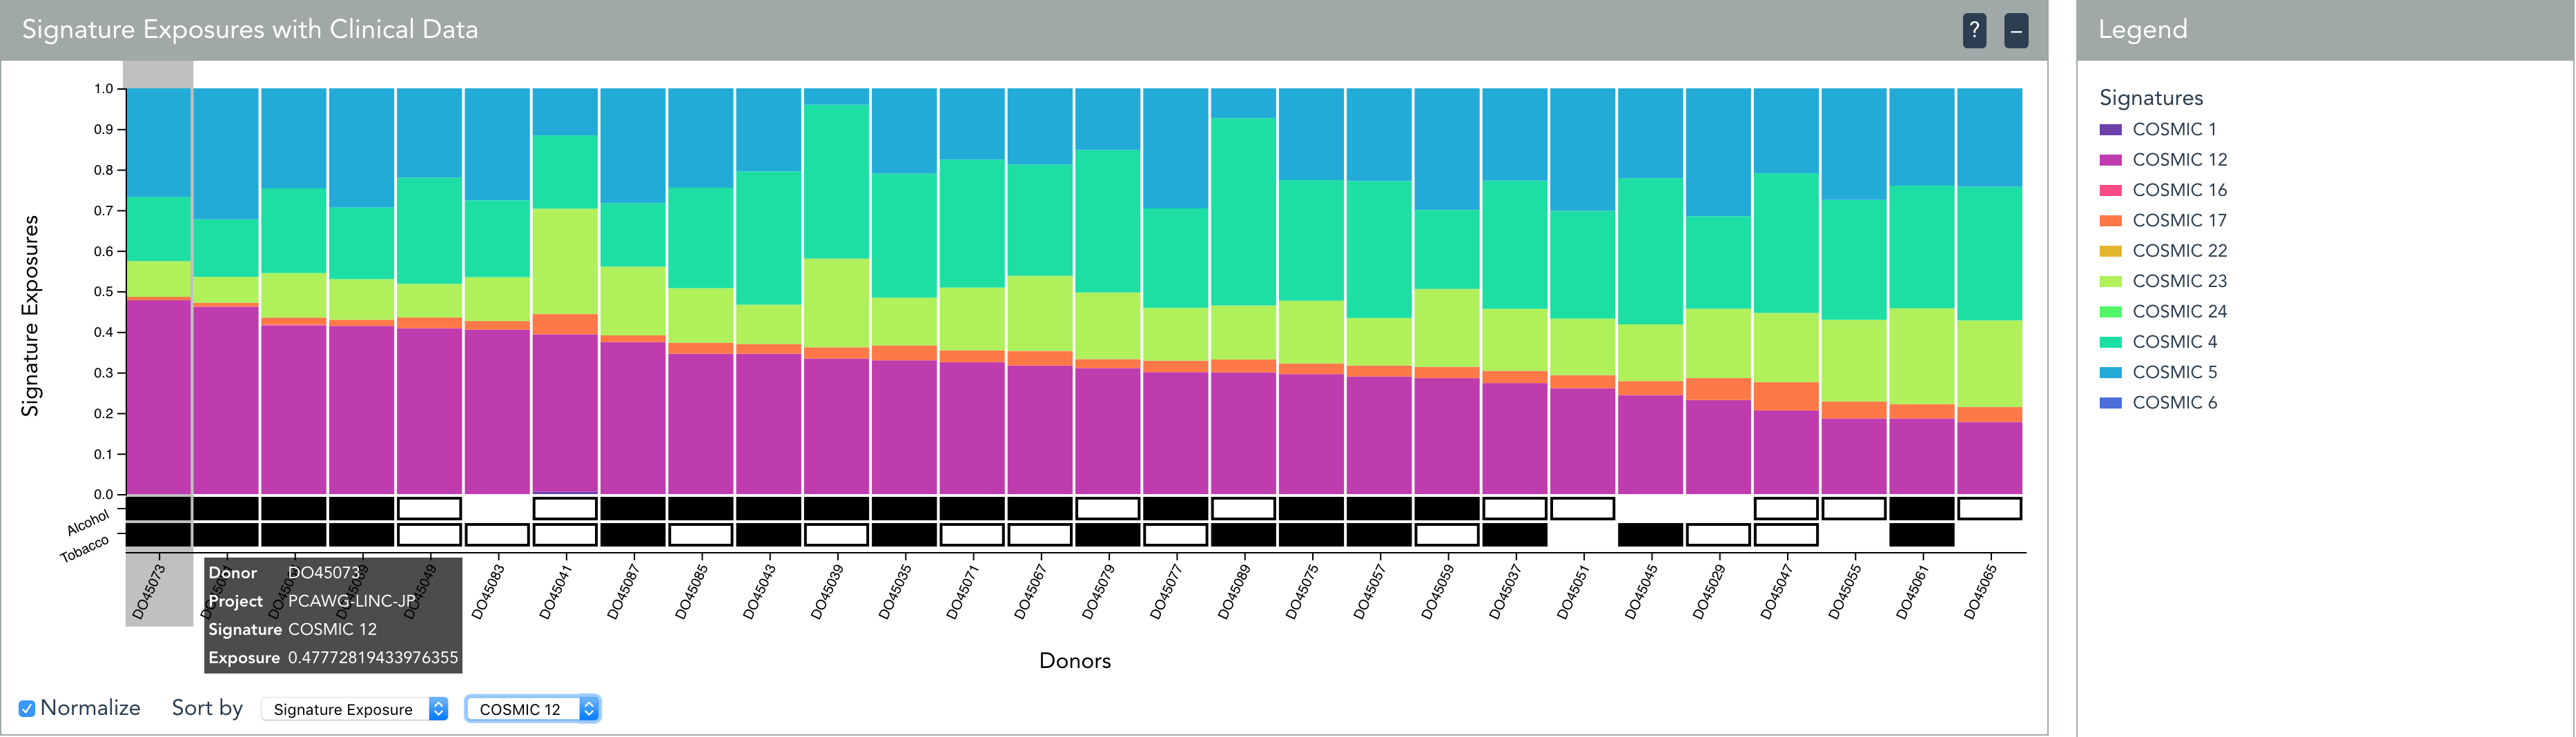
\includegraphics[width=0.75\columnwidth]{figures/case_study1.png}}
    \caption{Screenshot of Signature Exposures with Clinical Data plot with PCAWG-LINC-JP data, normalized and sorted by COSMIC signature 12}
    \label{fig:caseStudy1_sig12}
\end{figure}
Hovering over the samples and looking at the y-axis, we can see that the contribution of signature 12 ranges from over 10\% to just under 50\% for all samples.
Using this information, one could perform further statistical analysis on this data or seek out additional liver cancer mutation data to analyze.

Interestingly, when sorting by COSMIC signatures 1 and 16 - signatures both present in liver cancer and that resemble the \citet{li2018mutational} signature, a similar trend in alcohol usage arises (only two alcohol-free donors in the top half of donors).
However, the contributions from these two signatures are too low to be visible for any sample in the plot.
\subsection{Hypermutation and Mutation Category}
Another use case is the analysis of the relationship between hypermutation and mutation category.
For SNVs, the mutation category is the 5' flanking base pair, the mutation reference base pair, the variant base pair, and the 3' flanking base pair.

Mutations are assigned colors based on mutation categories on the rainfall plots to allow this type of relationship (or lack thereof) to be quickly spotted.
The prevalence of mutations with reference base C and 5' T in regions of kataegis is well documented \citep{taylor2013dna}.
\begin{wrapfigure}{r}{0.35\textwidth}
    \centering
    \frame{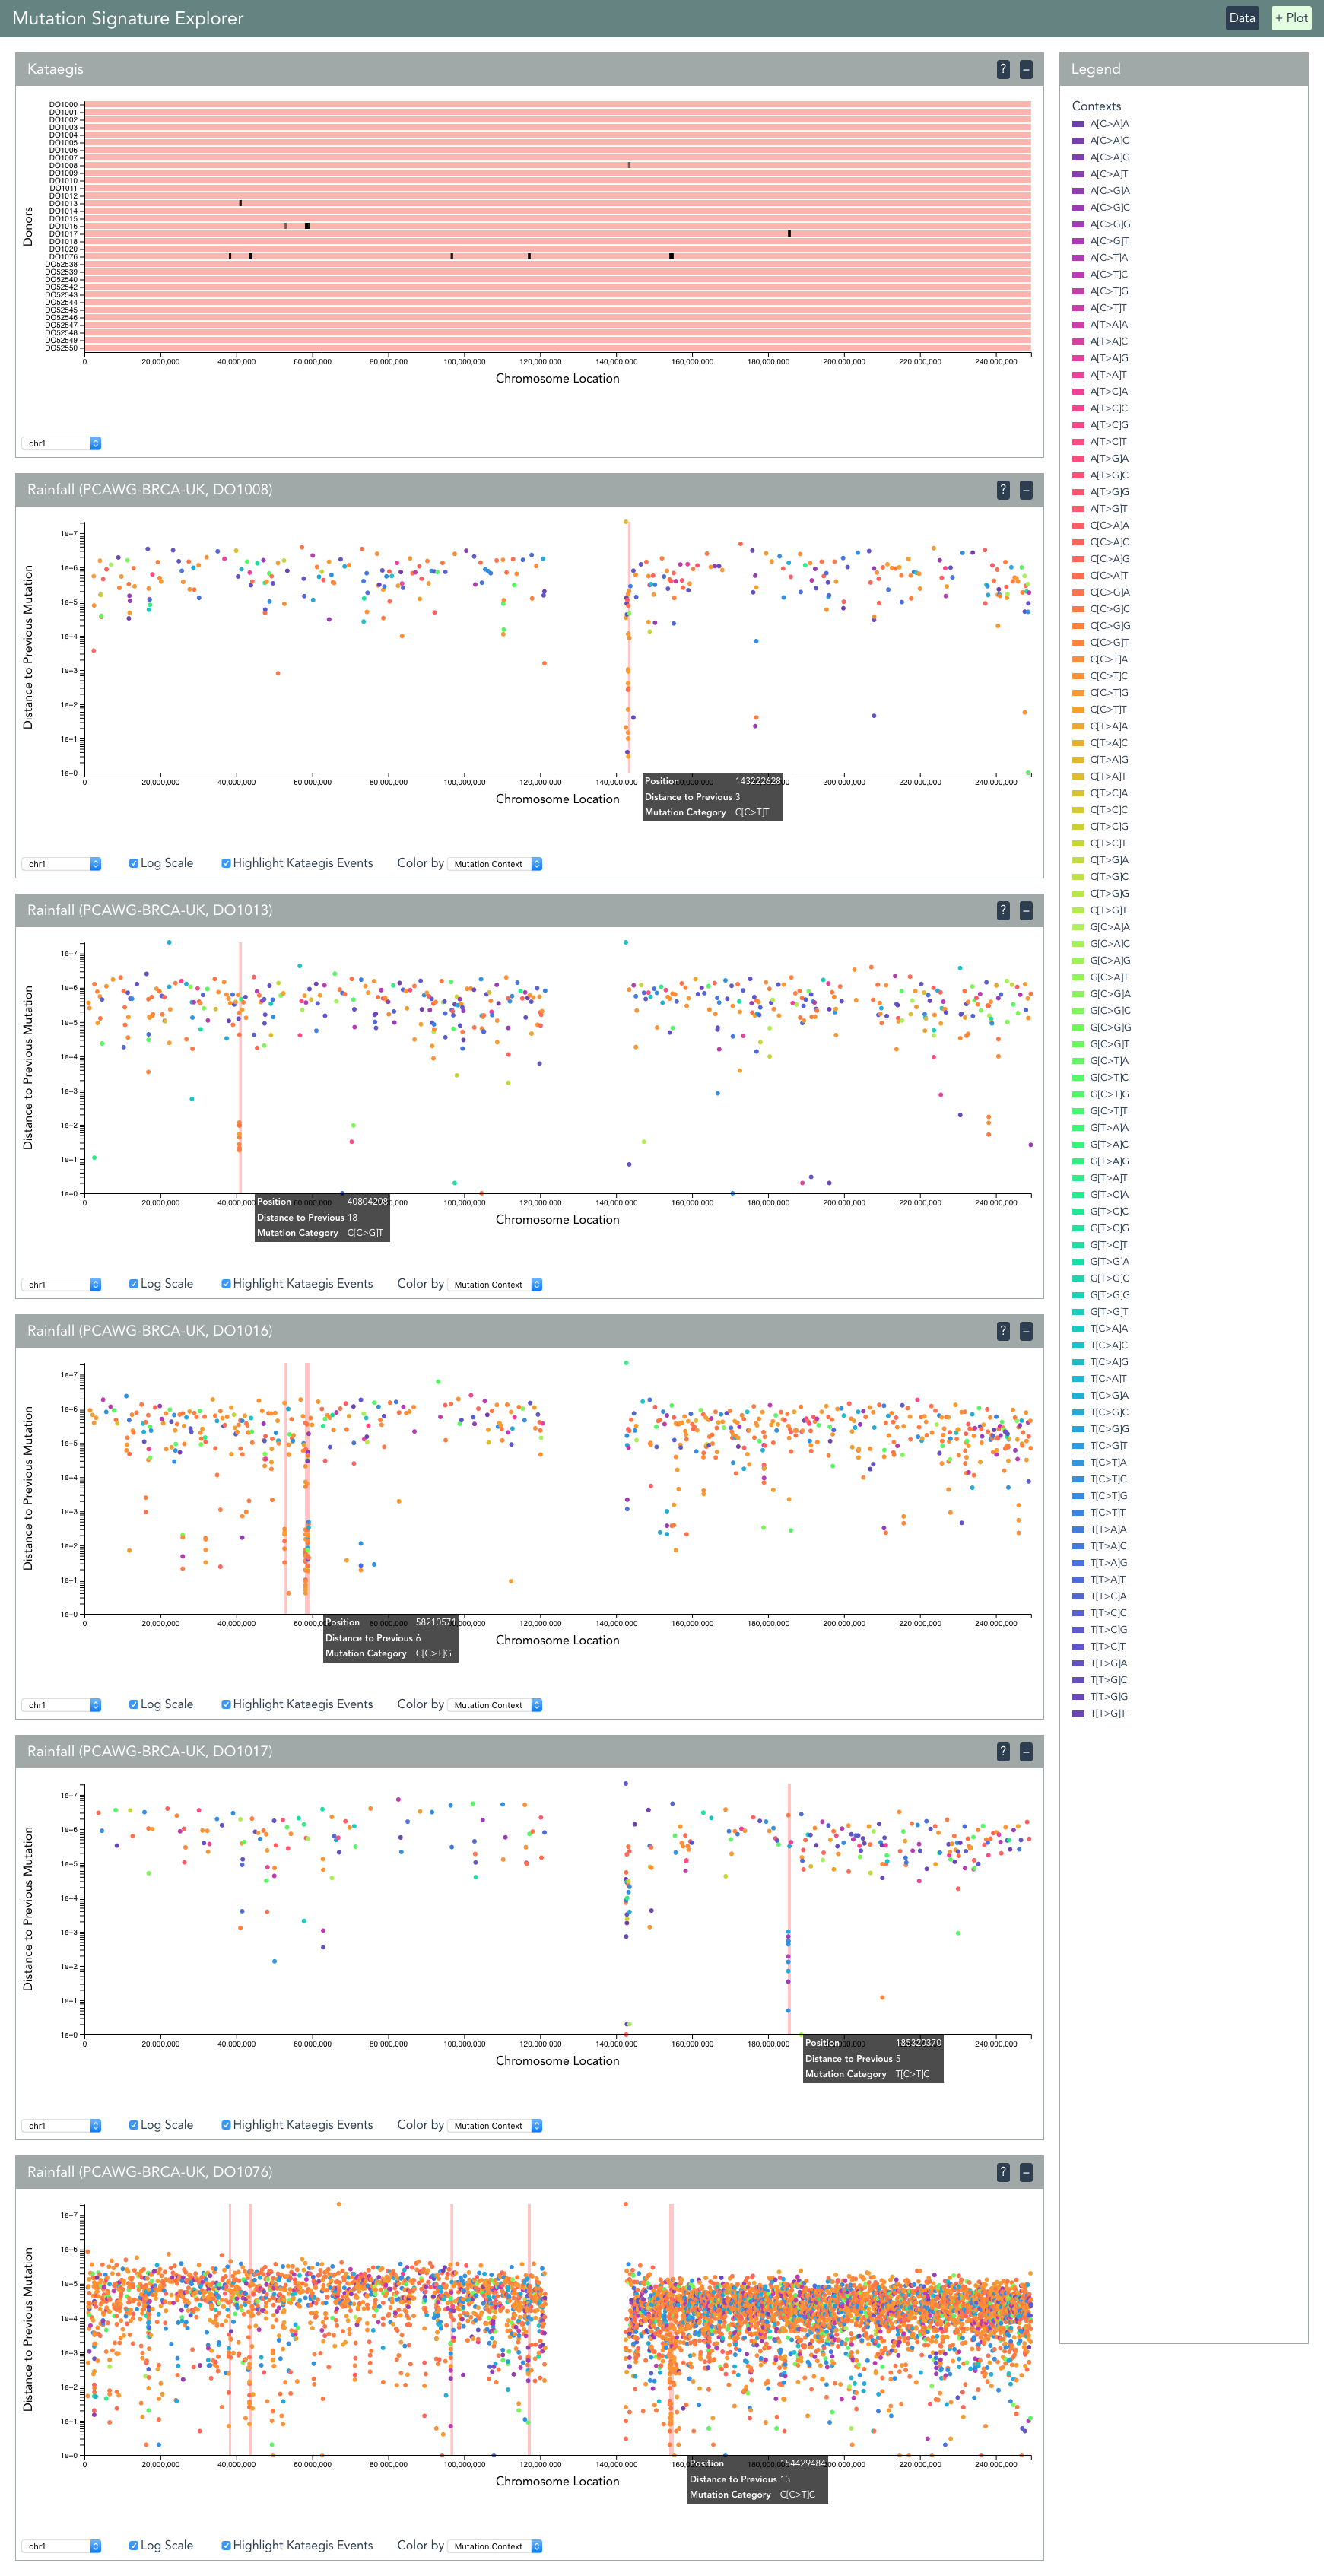
\includegraphics[width=0.33\textwidth]{figures/case_study2.png}}
    \caption{Screenshot of Rainfall Plots with PCAWG-BRCA-UK data for Chromosome 1}
    \label{fig:caseStudy2}
\end{wrapfigure}

To verify this relationship with iMuSE, we can choose the PCAWG UK Breast Triple Negative/Lobular Cancer cohort and add a Kataegis Plot.
Next, Rainfall Plots can be generated by choosing donors with kataegis events on chromosome 1.
By hovering over mutations in kataegis regions on these plots and looking at the categories on the legend, we see an abundance of orange-colored C[C\textgreater T]X mutations and some blue T[C\textgreater T]X mutations in these regions.
Figure \ref{fig:caseStudy2} shows these rainfall plots and the mutation category legend.
These plots could be used to discover further trends occurring in regions of hypermutation, such as significant rates of mutations that fall into categories with patterns other than T[C\textgreater T]X and C[C\textgreater T]X in specific cancer types.
Such discoveries can be communicated to others easily, as iMuSE URLs include information about current plot states.

% TODO: new case study on hypermutation regions not found by current approaches
\subsection{Discovery of Hypermutation Regions}
As previously mentioned, there have been recent efforts to better detect instances of kataegis \citep{yousif2018origins}.
\citet{alexandrov2013signatures} describes an early definition of kataegis as a set of 6 or more mutations with an average intermutational distance of less than 1,000 base pairs.
To understand why a more rigorous statistical definition of kataegis is needed, we can look at regions of hypermutation with iMuSE rainfall plots.
First, we can generate the kataegis plot for the PCAWG UK Breast Triple Negative/Lobular Cancer cohort and look at chromosome 1.
Selecting donor with ID DO1017, the rainfall plot shows one kataegis region, highlighted near location 180,000,000. 
But to the left of this, we see another kataegic event that is not highlighted because it was not detected by this method (Figure \ref{fig:caseStudy3}).
\begin{figure}[h]
    \centering
    \frame{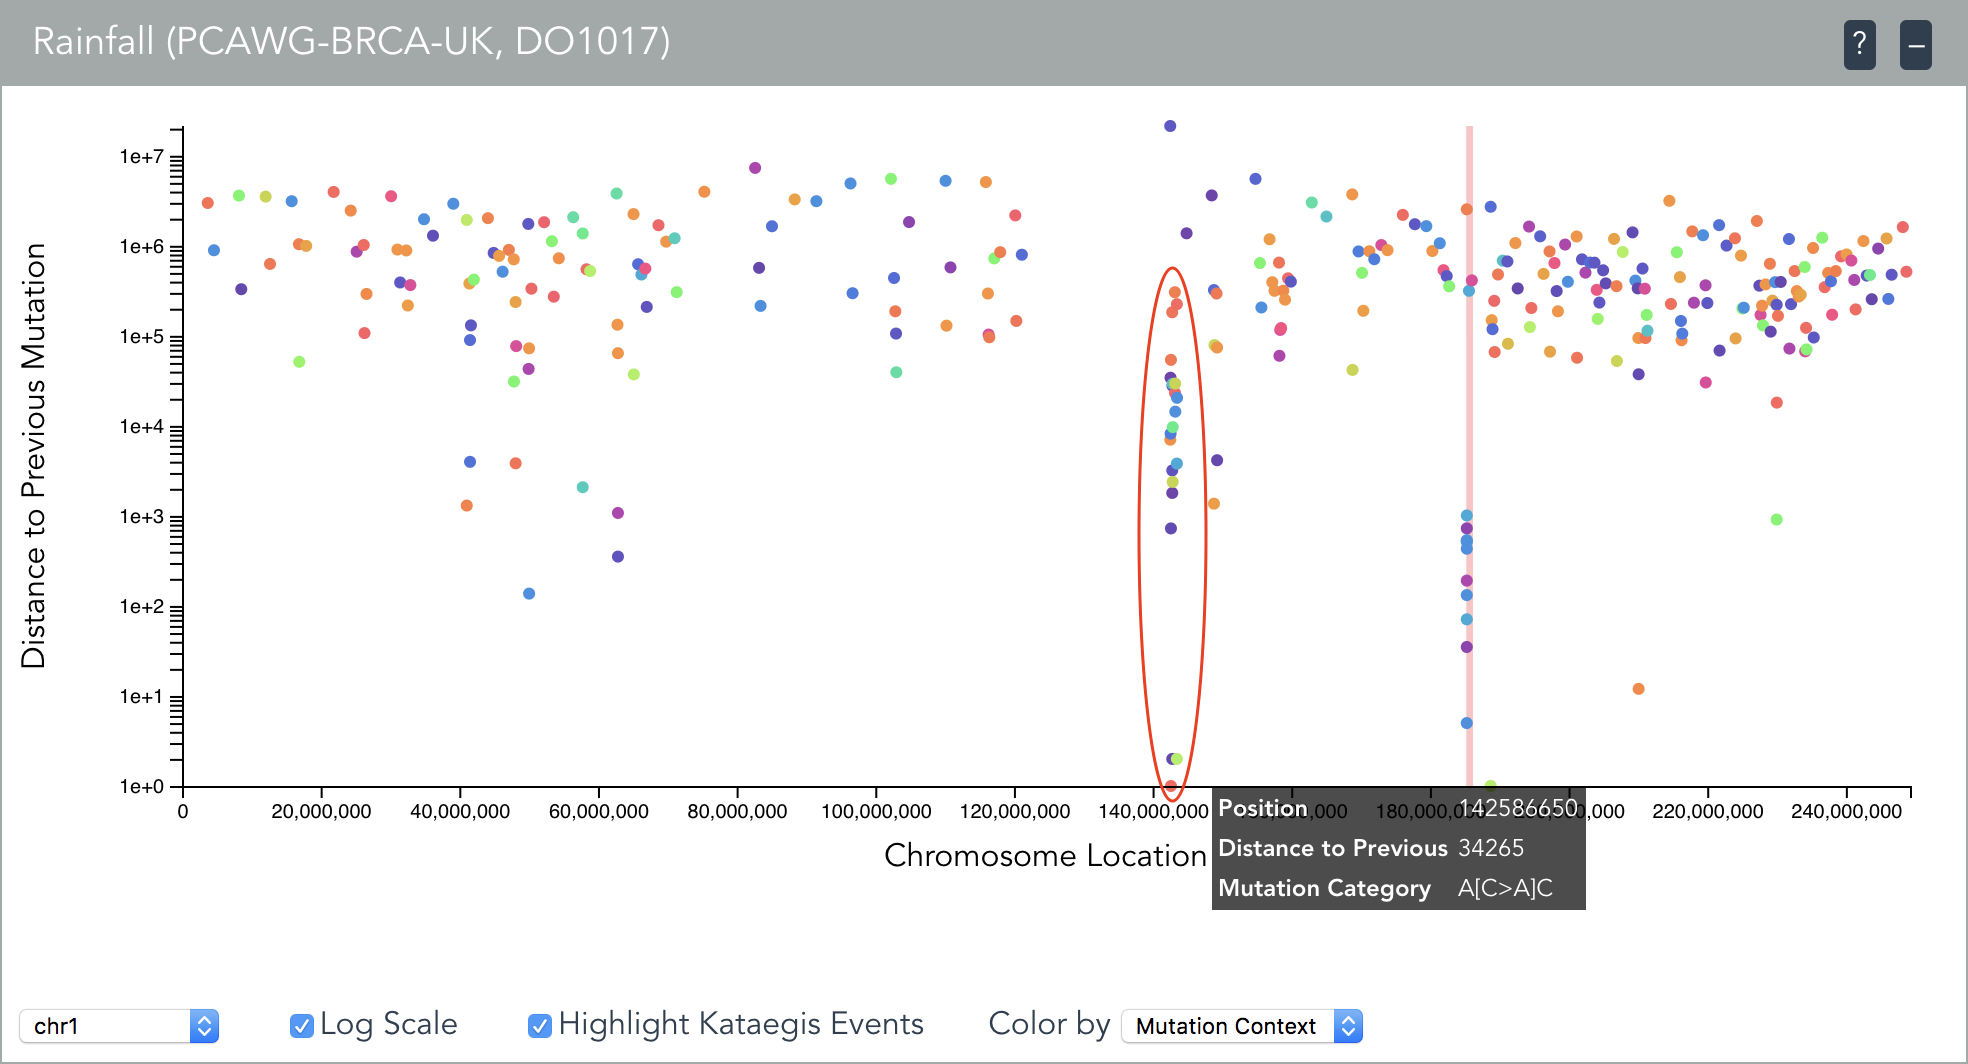
\includegraphics[width=0.75\columnwidth]{figures/case_study3.png}}
    \caption{Screenshot of Rainfall Plot with overlay identifying undetected kataegis region}
    \label{fig:caseStudy3}
\end{figure}


\section{Conclusions}
% Brief summary
In this paper, the motivations, features, design, and use cases of iMuSE, a web-based interactive visualization of mutational signature contributions, are presented. 
The ability to dynamically compute and visualize selected combinations of signatures, clinical variables, and cancer types makes this a powerful tool for data exploration.

% Future directions
Future development of iMuSE should focus on the addition of features that enable better analysis of single tumors. 
This could be implemented by allowing a user to trigger the creation of donor-specific visualizations in the same way that the rainfall plots are currently generated.
These features would help to better understand the processes acting in a single tumor.

Functionality can also be expanded through implementation of more plot types.
Specifically, visualization of mutational signatures themselves - as distributions over mutation categories - would be a simple but informative feature to add.
This would give users that are unfamiliar with mutational signatures a better sense of how the signatures are used in the other plot types.
These could look like interactive versions of the plots presented in Figure 2 of \citet{alexandrov2013signatures}.

Visualization of mutation rates, in the form of interactive mutational prevalence plots, should be used to show relationships between mutation rates and variables such as cancer type, clinical data, mutational signatures, and kataegis rates.
A mutation prevalence plot by cancer type is presented in Figure 1 of \citet{alexandrov2013signatures}.

Another Manhattan plot should be implemented, showing mutation rates along the genome by mutation category.

A plot showing the location of genes should be linked to existing plots that present data along the genome.
This type of plot showing gene locations can be found in Figure 1 of \citet{chelaru2014epiviz}.

Existing plots should be modified to allow analysis of mutation types other than SNVs. 
For example, since kataegis has been hypothesized to be associated with rearrangements, the rainfall and kataegis plots should be modified to show structural somatic mutations. The kataegis plot should also be modified to show survival status, which has also been hypothesized to be associated with kataegis.

Mutation datasets from additional sources should be processed to allow for stronger conclusions to be made using this tool.
When additional mutational signatures are discovered, they should be added to the database to ensure that users have access to the most relevant and accurate visualizations possible.
Local dataset visualization should be further enabled, to extend functionality beyond the public datasets we have processed.


\bibliography{main}{}
\bibliographystyle{plainnat}

\begin{figure}
    \centering
    \frame{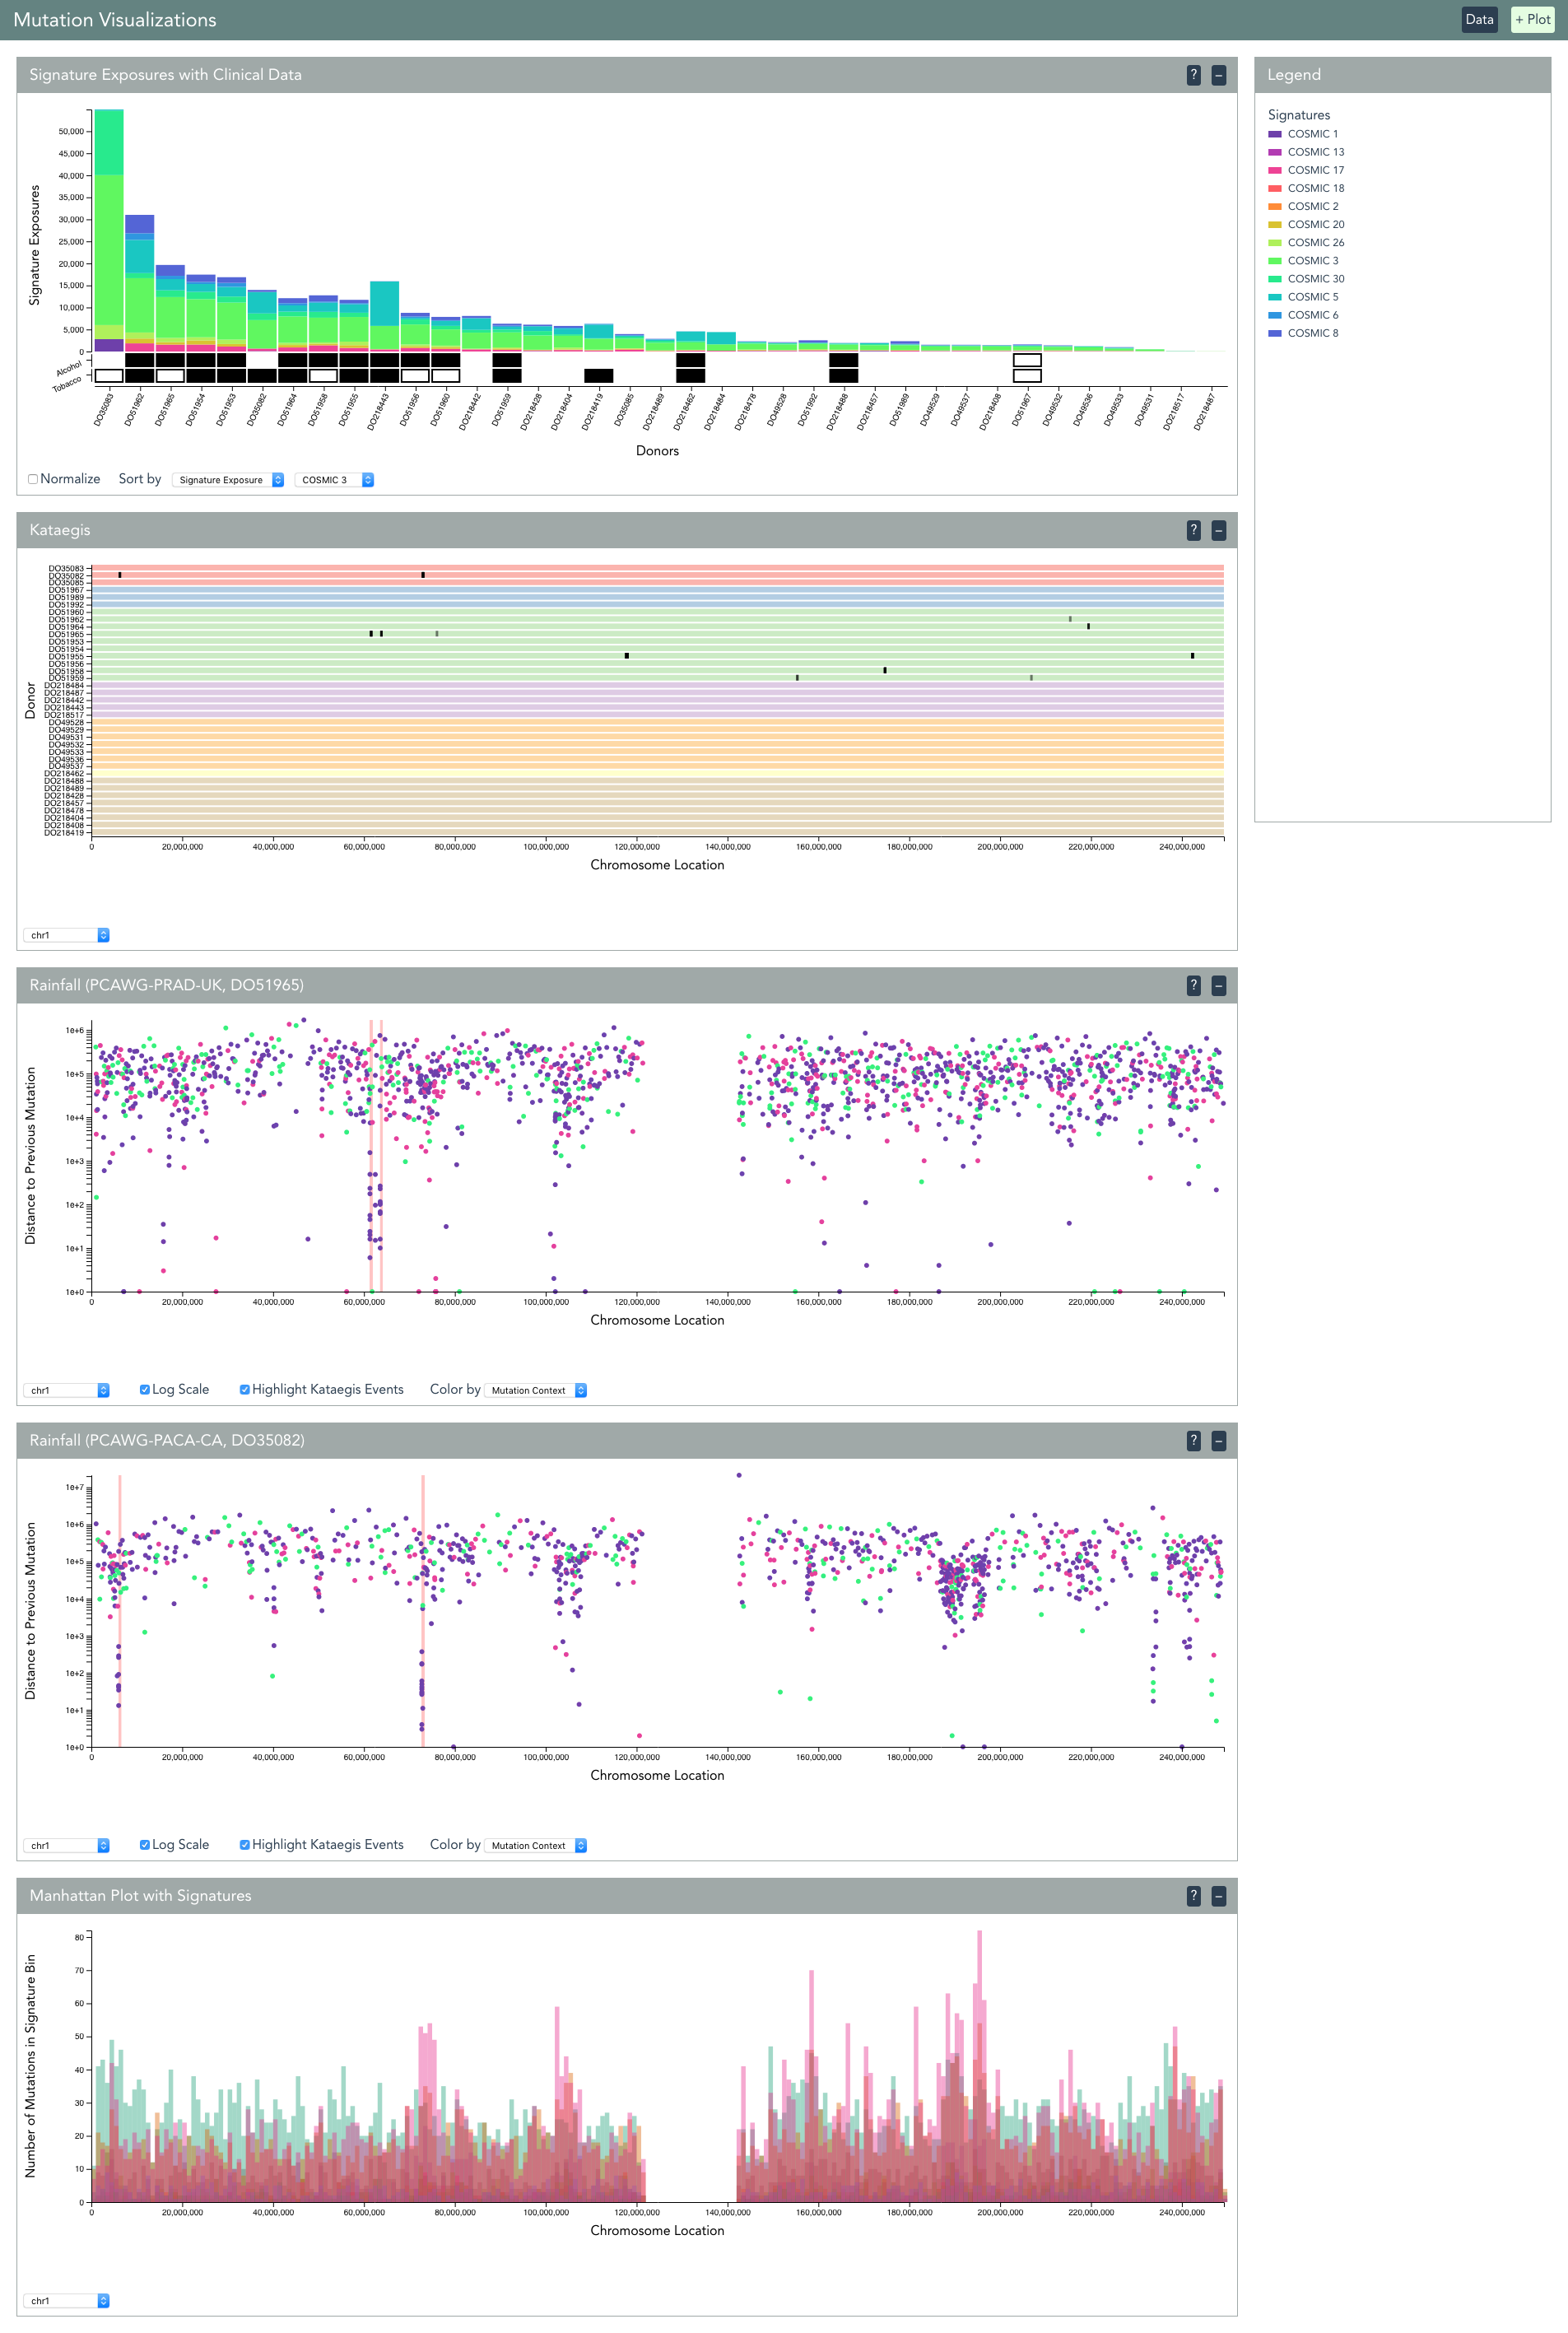
\includegraphics[width=0.75\columnwidth]{figures/screenshot1.png}}
    \caption{Screenshot displaying all plot types}
\end{figure}

\pagebreak

\appendix                                     
\section{Examples of Publication-Ready Figures}
\renewcommand{\figurename}{Example Figure}
\setcounter{figure}{0}

\begin{figure}[h!]
    \centering
    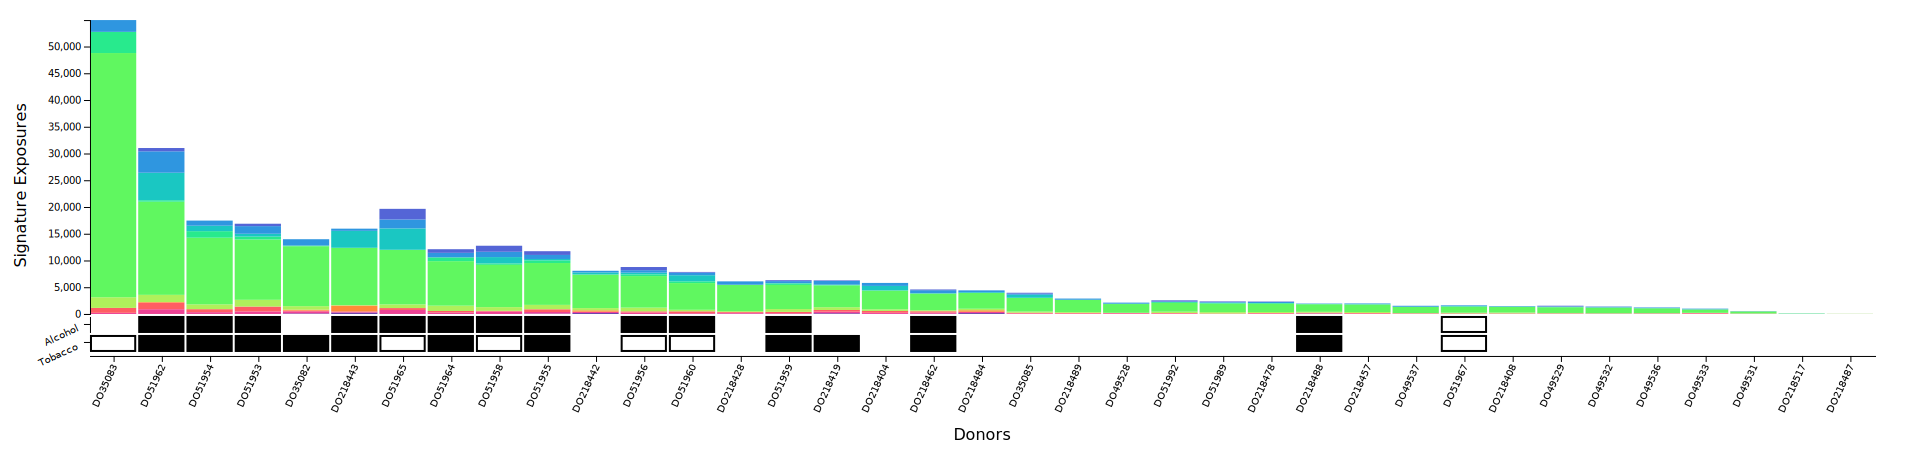
\includegraphics[width=\columnwidth]{figures/exposures.pdf}
    \caption{Signature Exposures with Clinical Variables}
\end{figure}
\begin{figure}[h!]
    \centering
    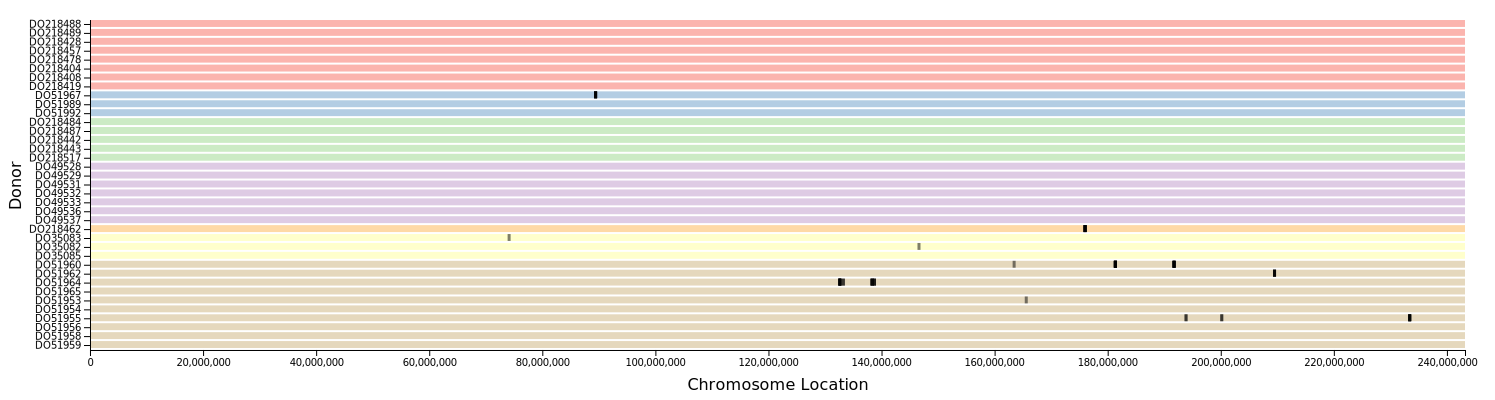
\includegraphics[width=\columnwidth]{figures/kataegis_chr2.pdf}
    \caption{Kataegis Plot (Chromosome 2)}
\end{figure}
\begin{figure}[h!]
    \centering
    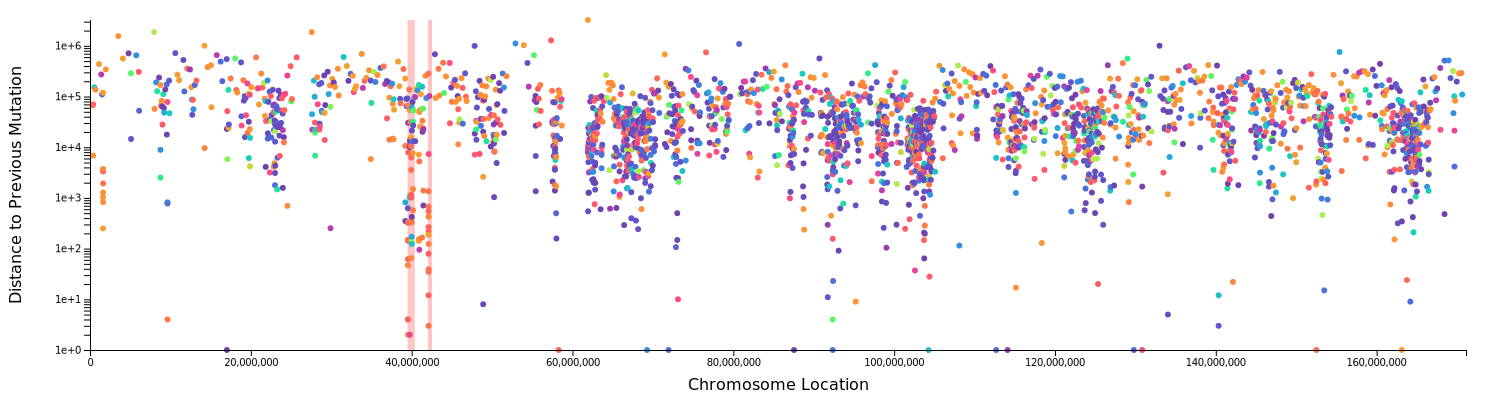
\includegraphics[width=\columnwidth]{figures/rainfall_DO50346_chr6.pdf}
    \caption{Rainfall Plot (Chromosome 6)}
\end{figure}
\begin{figure}[h!]
    \centering
    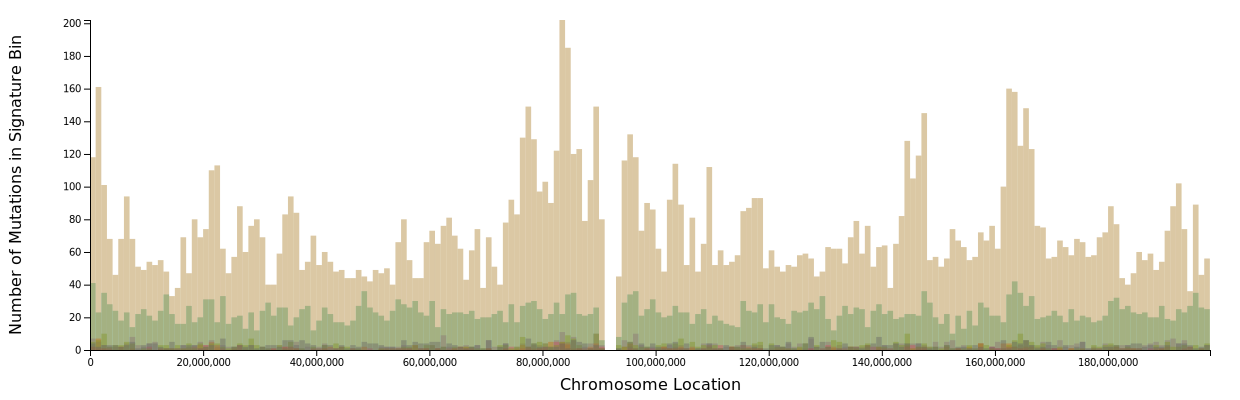
\includegraphics[width=\columnwidth]{figures/manhattan.pdf}
    \caption{Manhattan Plot (Chromosome 2)}
\end{figure}

\end{document}
